\documentclass[12pt,vu]{adammath}
\usepackage{preamble}

\begin{document}

\title{$p$-adic Numbers}
\abstracttitle{$p$-Adic Numbers}
\author[y.eshel@student.vu.nl, 2660535]{Yoav Eshel}
\author[vangianganh@gmail.com, 2658762]{Anh Van Giang}
\what{Project pure mathematics}
\programme{Bachelor Mathematics}
\track{Algebra and geometry}
\supervisor{prof.\ Rob de Jeu}
\coverimage{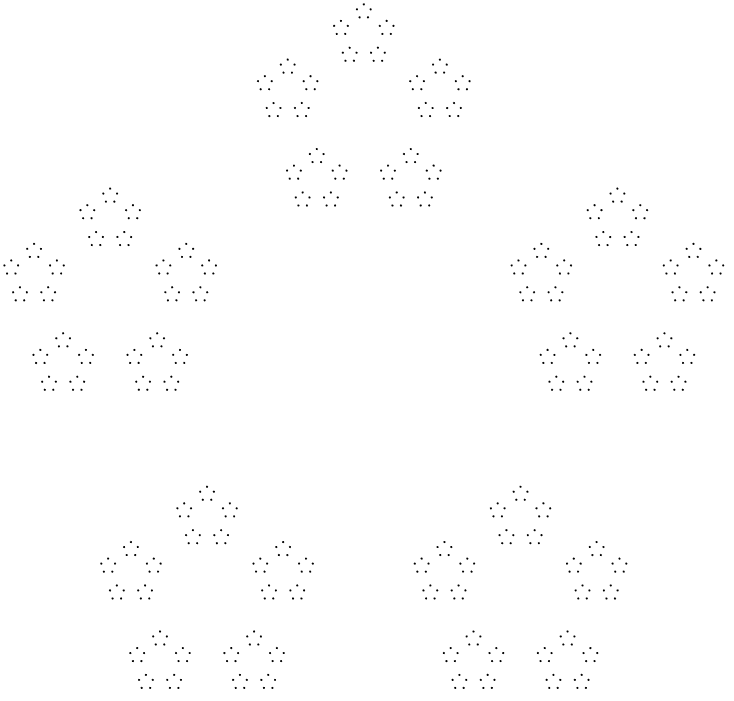
\includegraphics[scale=0.5]{cover-image}}
\maketitle

\frontmatter
\begin{abstract}
    The $p$-adic numbers and $p$-adic metric are introduced, and various relevant properties are proved. 
    The field $\Qp$ is then constructed as the completion of $\Q$ with respect to the $p$-adic absolute value and Hensel's lemma is proved using an iterative method.
    It is then shown that $\Qp$ is not algebraically closed and its algebraic closure is $\overline{\Qp}$ is not complete.
    The field $\Cp$ is constructed as the completion of the algebraic closure of $\Qp$ and Newton polygons are discussed as an example of analysis in $\Cp$.

    Cover image: a Euclidean model of $\Z_5$. Taken from \cite{Gouvea_2013}.
\end{abstract}

\begingroup
\tableofcontents
% \listoffigures
% \let\cleardoublepage\bigskip
% \let\clearpage\bigskip
% \listoftables
\endgroup
\printnomenclature

\mainmatter
\chapter{Introduction}
The $p$-adic numbers were first discovered\footnote{or invented, depending on your philosophical preferences} by Kurt Hensel in 1897 \cite{Gouvea_2013}, as a way to introduce the tools and techniques of power series into number theory.
Hensel started with the analogy between $\Z$ and its field of fractions $\Q$ and $\C[X]$ together with its field of fractions, $\C(X)$.
Both $\Z$ and $\C[X]$ are \textit{unique factorization domains}: any integers factors as $\pm1$ times the product of primes and any polynomial uniquely factors as a product of prime elements $X-\alpha\in\C[X]$.
Furthermore, any polynomial in $\C[X]$ can be expanded in "base" $X-\alpha$ using its Taylor series around $\alpha$ and for any integer $m\in\Z^+$ and prime $p$ we can write
\[m=a_0+a_1p+a_2p^2+\cdots+a_np^n,\quad a_i\in\{0,1,\dots, p-1\}.\]
There is also a natural expansion for $-1$, at least in a formal sense, as
\[-1=(p-1)+(p-1)p+(p-1)p^2+\cdots\]
since if we add $1$ we get
\begin{align*}
    0&=1-1\\
    &=1+(p-1)+(p-1)p+(p-1)p^2+\cdots\\
    &=p^2+(p-1)p^2+(p-1)p^3+\cdots\\
    &=0.
\end{align*}
Note that the powers of $p$ are disappearing "to the right".
The analogy gets interesting when we start considering rational numbers.
We know that every rational function in $\C(X)$ has an finite tailed Laurent series around $\alpha\in\C$ as
${P(X)}/{Q(X)}=\sum_{i\geq k}a_i(X-\alpha)^i$. Working formally, we can obtain a similar series for rational numbers.
For example, consider $p=3, a=22$ and $b=7$. Then $a=1+p+2p^2, b=1+2p$ and so
\begin{equation}\label{eq:p-adic-expansion}
    \frac{a}{b}=\frac{1+p+2p^2}{1+2p}=1-p+4 p^2-8 p^3+16 p^4-32 p^5+\cdots.
\end{equation}
It is easy to check that the above expansion is correct by multiplying both side by $b=1+2p$.

To make such expansions rigorous, we must define a new metric on $\Q$, such that larger powers of $p$ become increasingly small so that the series such as the one in (\ref{eq:p-adic-expansion}) actually converges.
This gives us the $p$-adic metric $\absp{\cdot}$ defined in section \ref{sec:p-adic-metric}. 
Furthermore, we know that every rational function has a Laurent expansion around $\alpha$, but not every Laurent expansion corresponds to a rational function (for example the Laurent series for $e^z$). 
This gives us the inclusion $\C(X)\hookrightarrow\C((X-\alpha))$ \nomenclature{$K((X))$}{field of finite-tailed formal power series with coefficients in $K$}. 
The field of all formal power series in $p$ is denoted $\Qp$ and is defined as the completion of $\Q$ with respect to $\absp{\cdot}$ in section \ref{sec:field-qp}.
After discussing an application of $p$-adic numbers to solving congruence relations modulo a prime $p$ in section \ref{sec:hensels-lemma} we move to the problem of construction a complete and algebraically closed field of $p$-adic numbers, analogous to the field $\C$ of complex numbers.

Using the standard norm on $\Q$, we can complete it to get the field $\R$ and then take the algebraic closure to end up with $\C$, a complete and algebraically closed field.
In the $p$-adic world, things get a bit more complicated. In chapter 3 we show that $\Qp$ is not algebraically closed and takes its algebraic closure $\overline{\Qp}$.
However, $\overline{\Qp}$ is not complete anymore, and so we take its completion again to get $\Cp$. We then prove that the completion of an algebraic closure of a complete field is always algebraically closed.
Finally, in chapter 4 Newton polygons are introduced as a way to analyze roots of polynomials and radius of convergence of power series.

\chapter{$p$-adic Numbers}
The expansion of a $p$-adic integer resembles the decimal expansion of a real number. 
However, the decimal expansion converges while the $p$-adic expansion might not. 
As the field of real numbers is the set of all decimal expansions, we can construct the field $\Qp$ of all $p$-adic expansions by replacing the ordinary absolute value with a $p$-adic one.

\section{$p$-adic absolute value}\label{sec:p-adic-metric}
Let $x=a/b\in\Q$ and $p$ prime. Then we can write $x=p^m\frac{a'}{b'}$ with $m\in\Z$ (or $m=\infty$ if $x=0$) and $\gcd(a'b', p)=1$.
The $p$-adic absolute value of $x$ is given by $\absp{x}=p^{-m}$ and is easily checked to verify the usual properties: 
\begin{itemize}
    \item $\absp{a}\geq 0$ and $\absp{a}=0\iff a=0$
    \item $\absp{ab}=\absp{a}\absp{b}$
    \item $\absp{a+b}\leq\absp{a}+\absp{b}$
\end{itemize}
for all $a,b\in\Q$.

The number $m$ associated with $x$ is called the $p$-adic valuation of $x$ and is denoted $\valp(a)$
This gives the map $\valp:\Q\to\Z\cup\{\infty\}$. We then have

\begin{prop}\label{prop:strong-ord}
The map $\valp:\Q\to\Z\cup\{\infty\}$ satisfies
\begin{enumerate}
    \item $\valp(x)=\infty\iff x=0$
    \item $\valp(xy)=\valp(x)+\valp(y)$
    \item $\valp(x+y)\geq\min\{\valp(x),\valp(y)\}$
\end{enumerate}
\end{prop}
\begin{proof}
    The first two properties are readily verified. For the third, if $x+y=0$ then $\valp(x+y)=\infty$ and the proof is trivial.
    So take $x,y\in\Q$ with $x+y\neq 0$ and without loss of generality, assume that $\valp(x)\leq\valp(y)$.
    Let $x=a/b$ and $y=c/d$. It is clear from the definition that $\valp(x)=\valp(a)-\valp(b)$ and so we have
    \[\valp(x)\leq\valp(y)\implies\valp(ad)\leq\valp(bc).\]
    Let $\valp(ad)=m$ and $\valp(bc)=n$. Then $ad+bc=p^mk_1+p^nk_2$ with $k_1,k_2\in\Z$ and since $m\leq n$ it follows that $p^m\mid ad+bc$.
    Thus $\valp(ad+bc)\geq\valp(ad)$ and so 
    \[\valp(x+y)=\valp\left(\frac{ad+bc}{bd}\right)=\valp(ad+bc)-\valp(bd)\geq\valp(a)-\valp(b)=\valp(x).\]
\end{proof}

From proposition \ref{prop:strong-ord} it follows that for $x,y\in\Q$ nonzero with $\valp(x)\leq\valp(y)$  and $x+y\neq0$ we have
\[\absp{x+y}=p^{-\valp(x+y)}\leq p^{-\valp(x)}=\absp{x}\]
and so $\absp{x+y}\leq\max\{\absp{x},\absp{y}\}$. By defining $p^{-\infty}=0$, the result extends to all of $\Q$.
Notice that this property is stronger than the usual triangle inequality, and so the $p$-adic absolute value is \textit{non-Archimedean}
as opposed to the ordinary absolute value on $\Q$. As one may expect, this property is quite unintuitive. 
For example, every point $a_2$ in an open disk $D(a_1, r)=\{x\in\Q\mid \absp{x-a_1}<r\}$ \nomenclature{$D(a,r)$}{open disk of radius $r$ centered at $a$} is its center.
That is becuase for any $x\in D(a_1, r)$ we have
\[\absp{x-a_2}=\absp{(x-a_1)+(a_1-a_2)}\leq\max\{\absp{x-a_1}, \absp{a_1-a_2}\}\leq r\]
so $x\in D(a_2, r)$. We can similarly show that $x\in D(a_2, r)$ implies that $x\in D(a_1,r)$ and so $D(a_1,r)=D(a_2, r)$.


\section{The field $\Qp$}\label{sec:field-qp}
From real analysis, we know that $\R$ is the completion of $\Q$ with repspect to a standard absolute value, i.e. $\R$ is a complete field, the absolute value in $\R$ is induced by the absolute value on $\Q$ and $\Q$ is dense in $\R$.
In this section we construct the field $\Qp$ as the completion of $\Q$ with repspect to $\absp{\cdot}$ in a similar manner. 
First recall that
\begin{definition}
A field $K$ with an absolute value $\abs{\cdot}$ is complete if every Cauchy sequence in $K$ has a limit in $K$.
\end{definition}
Due to Ostrowski, we know that there countably many non-equivalent\footnote{A more rigorous discussion what it means for two absolute values to be equivalent is found in Chapter 3. For now, an intuitive understanding of "equivalent" will suffice.} absolute values on $\Q$. Namely, the trivial absolute value which maps all non-zero elements to one, the ordinary absolute value and the $p$-adic absolute value(s) \cite[p. 46]{Gouvea_2013}.
As it turns out, $\Q$ is not complete with respect to any of its non-trivial absolute values. 
It is easy to show that $\Q$ is not compelte with repspect to the ordinary absolute value: consider the sequence given by $x_1=2$ and $x_n=\frac{1}{2}x_n+\frac{1}{x_n}$ which converges to $\sqrt{2}\not\in\Q$.
To show that $\Q$ is not complete with respect to the $p$-adic absolute value requires some more work. 
The following theorem is one of the many nice properties of non-Archimedean absolute values which will be used in showing that $\Q$ is not complete.
\begin{theorem}\label{thm:nonarch-cauchy}
Let $F$ be a field with a non-Archimedean norm $\abs{\cdot}$ and $\langle x_n \rangle$ a sequence in $F$. Then $\langle x_n \rangle$ is a Cauchy sequence if and only if 
$\lim_{n \rightarrow \infty} \abs{ x_{n+1} - x_n} = 0.$
\end{theorem}
\begin{proof}
The first implication is immidiate. Suppose that $\langle x_n\rangle$ is a sequence such that $\abs{x_{n+1}-x_n}\to0$.
Let $k > 0$ and $m = n + k$ then we have 
\begin{align*}
    \abs{ x_m - x_n} &= \abs{ x_{n+k} - x_{n+k-1} + x_{n+k-1} + ... - x_n }\\
    &\leq \max (\abs{x_{n+k} - x_{n+k-1}}, \abs{x_{n+k - 1} - x_{n+k-2}}, ..., \abs{x_{n+1} - x_n})\\
    &\leq \abs{x_{n+h} - x_{n+h-1}},\quad\text{for some $h \in \{1,2,...,k\}$}.
\end{align*}
As the last expression goes to 0 by assumption, $\langle x_n \rangle$ is Cauchy. 
\end{proof}


We can now prove that the field $\Q$ is not complete with respect to the $p$-adic absolute value.
\begin{theorem} 
    The field $\Q$ is not complete with respect to $\absp{\cdot}$.
\end{theorem}
\begin{proof}
If $p\in\{2,3\}$, the proof is more complicated and requires Hensel's lemma. A sketch of the proof is given in the end of section \ref{sec:hensels-lemma}.

Suppose $p>3$. Let $1<a<p-1$ and define the sequence $x_n=a^{p^n}$.
Then 
\[\absp{x_{n+1}-x_n}=\absp{a^{p^n}\left(a^{(p-1)p^n}-1\right)}\leq p^{-n}\]
where the last inequality follows from Euler's theorem as $a^{(p-1)p^n}=a^{\phi(p^n)}\equiv 1\mod p^n$. Thus $\langle x_n\rangle$ is a Cauchy sequence.
Suppose that $x_n\to x\in\Q$. Since the roots of $X^p-X$ are the $\frac{p-1}{2}$th primitive roots of unity, $\pm 1$ and $0$, it follows that $x=0,\pm1$.
As $p\nmid a^{p^n}$ for all $n$, $\absp{x_n}=1$ for all $n$, and so $\absp{x}=\lim_{n\to\infty}\absp{x_n}=1$. Thus $x\neq 0$.
If $x=\pm 1$, then $0<x-a<p$ and so $\absp{x-a}=1$. Thus there exists $n\in\N$ such that $\absp{a^{p^n}-x}<\absp{x-a}$.
It is easy to check that $\absp{x-a}\leq\max\{\absp{x-a^{p^n}},\absp{a^{p^n}-a}\}$ implies that $\absp{x-a}=\absp{a^{p^n}-a}$.
But $\absp{a^{p^n}-a}=\absp{a^{p^{n-1}}-1}$ and by Fermat's little theorem we have $a^{p^{n-1}}-1\equiv0\mod p$ so $\absp{x-a}<1$, contradicting our previous assertion.
Thus $x\not\in\Q$ and it follows that $\Qp$ is not complete with respect to the $p$-adic norm for all primes $p$.
\end{proof}

We now know that $\Q$ is not complete, but it is unclear how to obtain a complete extension of $\Q$, and in particular, how does the $p$-adic absolute value extends.
It turns out that one can mimic the Cauchy construction of $\R$ by letting $\Qp$ be the set of equivalence classes of Cauchy sequences in $\Q$ with respect to the $p$-adic norm. The proof is adapted from \cite[p. 468]{lang_02}.

\begin{theorem}\label{thm:unique-completion}
Let $K$ be a field with an absolute value $\abs{\cdot}$. 
Then there exists a field $K'$ with an absolute value $\abs{\cdot}'$ and an embedding $i:K\to K'$ such that $\abs{i(x)}'=\abs{x}$ for $x\in K$ and the image of $K$ is dense in $K'$.
The field $K'$ is unique up to isomorphism. Moreover, if $\abs{\cdot}$ is non-Archimedean, then $\abs{\cdot}'$ is non-Archimedean.
\end{theorem}
\begin{proof} 
    The set $R$ of Cauchy sequences in $K$ forms a ring, with addition and multiplication defined componentwise.
    We call a sequence $\langle x_n\rangle$ a \textit{null sequence}, if $x_n\to 0$. 
    As any Cauchy sequence that is not null, will stay away from 0 for sufficiently large $n$, we can then take the inverse of almost all the terms. For finitely many of them, we again obtain a Cauchy sequence.
    Thus the set of all null-sequences $M$ forms a maximal ideal in $R$. 
    
    We then define $K'$ as $R/M$ and the embedding $i$ is the map sending $x\in K$ to the class of constant Cauchy sequences $(x,x,\dots)$.
    The absolute value $\abs{\cdot}'$ is defined by continuity, i.e. for an element $\alpha\in K'$ representing a sequence $\langle x_n\rangle$ we have $\abs{\alpha}'=\lim_{n\to\infty}\abs{x_n}$.
    This limit exists since $\abs{\abs{x_n}-\abs{x_m}}\leq\abs{x_n-x_m}$ implies that $\abs{x_n}$ is a Cauchy sequence in $\R$. 
    It is immediate that $\abs{\cdot}'$ has the usual properties independently of the choice of $x_n$ and that $\abs{i(x)}'=\abs{x}$ for all $x\in K$. 
    If $\abs{\cdot}$ is non-Archimedean, then for $\alpha,\beta\in K'$ representing the sequences $\langle x_n\rangle, \langle y_n\rangle$ (respectively) in $K$, we have
    \[\absp{\alpha+\beta}'=\lim\abs{x_n+y_n}\leq\lim\max\{\abs{x_n}, \abs{y_n}\}=\max\{\abs{\alpha}',\abs{\beta}'\}.\]

    To show that $K'$ is complete, let $\alpha_n$ be a Cauchy sequence in $K'$. Then there exist $x_n\in K$ such that $\abs{\alpha_n-i(x_n)}'<\frac{1}{n}$. 
    The sequence $x_n$ forms a Cauchy sequence in $K$ with a limit $\alpha\in K'$. As
    \[\abs{\alpha_n-\alpha}'\leq\abs{\alpha_n-i(x_n)}'+\abs{i(x_n)-\alpha}'\]
    it follows that $\alpha_n\to\alpha$ and so $K'$ is complete. 

    For any $\alpha\in K'$ represented by a sequence $\langle x_n\rangle$ in $K$, there exists an $x_N$ for $N \in \N$ so that $i(x_N)$ is arbitrarily close to $\alpha$ and so $i(K)$ is dense in $K'$.
    Finally, uniqueness is immediate, since for any complete field $\hat{K}$ that contains $K$ as a dense subfield, we can map limits in $\hat{K}$ of Cauchy sequences in $K$ to their representatives in $K'$. 
\end{proof}

Thus the extension $\Qp/\Q$ exists and is unique, and there is a well defined absolute value on $\Qp$ which is induced by the $p$-adic absolute value on $\Q$.
As a result, we will denote the absolute value on $\Qp$ as $\absp{\cdot}$ as well.

Let $K$ be a complete field w.r.t. a non-Archimedean absolute value $\abs{\cdot}$. 
Let $\mcO_K=\{x\in K\mid \abs{x}\leq 1\}$. It is immediate from the properties of non-Archimedean absolute values that $\mcO_K$ is a ring. 
We calle this the valuation ring of $K$. 
Similarly, it can be found that $M=\{x\in K\mid \abs{x}<1\}$ is an ideal of $\mcO_K$. 
To show that $M$ is the unique maximal ideal of $\mcO_K$, take $\alpha\in\mcO_K\setminus M$. Then $\abs{\alpha}=1$ so $\abs{\alpha^{-1}}=1$ and it follows that any ideal containing $\alpha$ must be the whole ring. 
If $K$ is complete and $\langle x_n\rangle$ is a Cauchy sequence in $\mcO_K$ with limit $x\in K$, then $\abs{x_n}$ is a Cauchy sequence in $[0,1]$ and so $x\in\mcO_K$.
We summarize our results in the following proposition.
\begin{prop}
    Let $K$ be field with a non-Archimedean absolute value $\abs{\cdot}$.
    The subset $\mcO_K=\{x\in K\mid \abs{x}\leq 1\}$
    is a ring with a unique maximal ideal $M=\{x\in K\mid \abs{x}<1\}$.
    If $K$ is complete, then $\mcO_K$ is complete.
\end{prop}
\nomenclature{$\mcO_K$}{valuation ring of a field $K$}

The valuation ring of $\Qp$ is called the $p$-adic integers and denoted by $\Z_p$.

\section{Hensel's Lemma}\label{sec:hensels-lemma}
At this point, the only understanding we have of $p$-adic numbers is that their are limits of Cauchy sequences in $\Q$. 
Recall that we can write any rational number as a $p$-adic expansion, but not every $p$-adic expansion corresponds to a rational number.
This is analogous to the inclusion $\C(X)\hookrightarrow C((X-\alpha))$ of the field of rational functions to the field of finite-tailed Laurent series in $(X-\alpha)$.
Let $K$ denote the field of all elements of the form $\sum_{i\geq k} a_i p^i, a_i\in\{0,1,\dots,p-1\}$ where $k\in\Z$ and $a_k\neq 0$. 
It is clear that for any $\alpha\in K$,  $\alpha\in\Qp$ since the partial sums form a Cauchy sequence in $\Q$ and that for $\alpha\in K$, $\absp{\alpha}=p^{-k}$.
If $\alpha_n=\sum_{i\geq k_n} a_i^{(n)}p^i$ forms a Cauchy sequence in $K$, then the partial sums $x_n=\sum_{i=k_n}^{n-1}a_i^{(n)}p^i$ form a Cauchy sequence in $\Q$ with a limit $\alpha\in\Qp$. Then
\[\absp{\alpha_n-\alpha}\leq\max\{\absp{\alpha_n-x_n}, \absp{x_n-\alpha}\}=\max\{p^{-n}, \abs{x_n-\alpha}\}.\]
Thus $K$ is complete and so

\begin{prop}
For every $\alpha\in\Qp$ there exists $k\in\Z$ such that
\[\alpha=\sum_{i\geq k}a_ip^i,\quad a_i\in\{0,1,\dots, p-1\}, a_k\neq 0\]
and $\valp(\alpha)=k$. Conversely, for every $k\in\Z$ there exists $\alpha\in\Qp$ with $\valp(\alpha)=k$.
\end{prop} 

We are now ready to prove Hensel's lemma, which is one of the most important theorems of $p$-adic numbers. Using Hensel's lemma, we can, in many cases, quite easily determine whether a polynomial has a roots in $\Zp$.
There are in fact many forms of Hensel's lemma, and we give here the proof of only one, together with a more general statement which we will not prove here.
The idea is that in $\R$, we can sometime decide on the existence of roots by looking at the sign of a polynomial. For example, since $x^2+1>1$ for all $x\in\R$, $\R$ is not algebraically closed.
In the $p$-adic world, this translates to reduction $\mod p$. The following proof is adapted from \cite[p. 89]{Gouvea_2013}.

\begin{theorem} 
    Let $P(X) = a_nX^n+a_{n-1}X^{n-1}+\cdot+a_0$ be a polynomial with coefficients in $\Zp$. 
    Suppose that there exists $\alpha_1 \in \Z_p$ such that $P(\alpha_1)\equiv 0\mod p\Zp$ and $P'(\alpha_1)\not\equiv 0\mod p\Zp$ where $P'$ is the formal derivative of $P$. 
    Then there exists a unique $\alpha \in \Z_p$ such that $\alpha \equiv \alpha_1\mod p\Z_p$ and $P(\alpha) = 0$.
\end{theorem}
\begin{proof}
    We construct a unique Cauchy sequence $\langle \alpha_n\rangle$ in $\Zp$ such that for all $n \geq 1$: (a) $P(\alpha_n) \equiv 0\mod p^{n}$ and (b) $\alpha_n \equiv \alpha_{n-1}\mod p^{n}$.
    
    We assume that $\alpha_1$ exists. To find $\alpha_2$, note that by condition (b) it must be of the form $\alpha_2=\alpha_1+b_1p$, for $b_1\in\Zp$.
    Using the Taylor expansion of $P(X)$ around $\alpha_1$ we obtain
    \begin{align*}
        P(\alpha_2)&=P(\alpha_1+b_1p)\\
        &=P(\alpha_1)+P'(\alpha_1)b_1p+\text{terms divisible by }p^2\\
        &\equiv P(\alpha_1)+P'(\alpha_1)b_1p\mod p^2.
    \end{align*}
    Thus we need $b_1$ such that $P(\alpha_1)+P'(\alpha_1)b_1p\equiv 0\mod p^2$. From $P(\alpha_1)\equiv 0\mod p$ it follows that $P(\alpha_1)=px$ for some $x\in\Zp$ and so $x+P'(\alpha_1)b\equiv 0\mod p$. 
    As $P'(\alpha_1)$ is not divisible by $p$, it is invertible in $\Zp$ and so $b_1\equiv -x\left(P'(\alpha_1)\right)^{-1}\mod p$.
    Such $b_1$ exists in $\{0,1,\dots, p-1\}$, and for such $b_1$ we can set $\alpha_2=\alpha_1+b_1p$ satisfying both conditions.

    Exactly the same procedure can be taken to obtain $\alpha_{n+1}$ from $\alpha_n$ (and choosing $b_n$ in $\{0,1,\dots, p^n-1\}$) and so our sequence exists. As $\alpha_{n+1}-\alpha_n\equiv 0\mod p^n$ it follows that $\absp{\alpha_{n+1}-\alpha_n}\leq p^{-n}$ and so $\langle \alpha_n\rangle$ is Cauchy and it has a limit $\alpha\in\Zp$.
    Moreover, we have $P(\alpha)=0$ by continuity and so the proof is complete.
\end{proof}

We will need a more general version of Hensel's Lemma to prove that $\absp{\cdot}$ extends uniquely to algebraic extensions of $\Qp$, and so we note it here. The proof can be found in \cite[p. 129]{jurgen_99}
\begin{lemma}\label{lemma:gen-hensel}
    Let $K$ be a field with equipped with a non-Archimedean absolute value $\abs{\cdot}$, a valuation ring $\mcO_K$ and it maximal ideal $M$. 
    If a primitive polynomial $f\in\mcO_K[X]$ admits modulo $M$ factorization $f=\bar{g}\bar{h}\mod M$ into relatively prime polynomials $\bar{g},\bar{h}\in\mcO/M[X]$, then $f$ admits a factorization $f=gh$ into polynomials $g,h\in\mcO_K[X]$ such that $\deg g=\deg\bar{g}$, $g\equiv\bar{g}\mod M$ and $h\equiv\bar{h}\mod M$
\end{lemma}

One may see that the proof technique used is quite similar to Newton's method for find real root of a polynomial. 
We find $\alpha_{n+1}$ by solving $b_n=-x\left(P'(\alpha_n)\right)^{-1}$ so putting it all together we get 
\[\alpha_{n+1}=\alpha_n-p\frac{P(\alpha_n)}{p}\left(P'(\alpha_n)\right)^{-1}=\alpha_n-\frac{P(\alpha_n)}{P'(\alpha_n)}.\]
\begin{example} 
We show that the "square root" of 2\footnote{Meaning, a root of $X^2-2\in\Zp[X]$} is in $\Z_7$. Let $f(X)=X^2-2$. Then modulo 7, 3 and 4 are roots so let $\alpha_1=3$.
Then $f(\alpha_1)=7$ and $f'(\alpha_1)=6$. As $6^{-1}\equiv 41\mod 7^2$, we have
\[\alpha_1-\frac{f(\alpha_1)}{f'(\alpha_2)}=\frac{11}{6}\equiv 10\mod 7^2.\]
So $\alpha_2=10=3+1\cdot 7$
Continuing in the same manner we find that $\alpha_3=108=3+1\cdot 7+2\cdot 7^2$ and so on. Thus the square root of 2 in $\Z_7$ has an initial expansion $3+1\cdot 7+2\cdot 7^2+6\cdot 7^3+\cdots$.
\end{example}

Another application of Hensel's lemma is proving that $\Q$ is not complete with respect to $\absp{\cdot}$ when $p=2,3$. The polynomial $X^3+3$ is irreducible over $\Q[X]$ but it has a root modulo 2. 
Thus by Hensel's lemma it has a root in $\Z_p$ and it follows that $\Q$ is a proper subset of $\Q_2$ so $\Q$ cannot be complete. A similar argument using the polynomial $X^2+2$ when $p=3$ does the trick.
\chapter{Complete and Algebraically Closed Extension of $\Qp$}
The aim of the following chapter is to construct the field $\Cp$, a complete and algebraically closed extension of $\Qp$. This field takes the role of the complex numbers $\C$ in the $p$-adic world. We start by proving that $\Qp$ is not algebraically closed by showing that $\sqrt{p}\not\in\Qp$.
\begin{prop}
    The field $\Qp$ is not algebraically closed.
\end{prop}
\begin{proof}
    Suppose there exists $x\in\Qp$ such that $x^2=p$. Then
    $2\valp{(x)}=\valp{(x^2)}=\valp{(p)}=1.$
    As the $p$-adic valuation on $\Qp^\times$ is always an integer, we have a contradiction. Thus $x\not\in\Qp$ and so $\Qp$ is not algebraically closed.
\end{proof}
Before we can move on to the algebraic closure $\overline{\Qp}$ of $\Qp$, we need to show that the $p$-adic value can, in fact, be extended to $\overline{\Qp}$, 
\nomenclature{$\overline{K}$}{algebraic closure of a field $K$}
\section{Extensions of absolute values}
Let $K$ be a complete field equipped with an absolute value $\abs{\cdot}$. Before proving that $\abs{\cdot}$ can be uniquely extended to algebraic extensions of $K$, we define what it means for two absolute values to be equivalent.
\begin{definition}
    Two absolute values $\abs{\cdot}_1$ and $\abs{\cdot}_2$ on a field $K$ are called equivalent if they define the same topology on $K$.
\end{definition}
An alternative and more useful definition is given by the following proposition, the proof of which is due to \cite[p. 117]{jurgen_99}.
\begin{prop}
    Two non-trivial absolute values $\abs{\cdot}_1$ and $\abs{\cdot}_2$ on a field $K$ are equivalent if and only if
    \[\abs{\alpha}_1<1\implies\abs{\alpha}_2<1\]
    for $\alpha\in K$.
\end{prop}
\begin{proof}
    Suppose the two absolute values are equivalent. For $x\in K$ we have $\abs{x}_1<1$ if and only if $x^n\to 0$ as $n\to\infty$. As $\abs{\cdot}_1$ and $\abs{\cdot}_2$ define the same topology on $K$, it follows that $\abs{x}_2<1$ as well.

    Conversely, suppose that $\abs{x}_1<1\implies\abs{x}_2<1$.
    As both absolute values are non trivial, there exists $x_0\in K$ such that
    $\abs{x_0}_1>1$. Then $\abs{x_0}_2>1$ since $\abs{x_0^{-1}}_1<1$. Let $a=\abs{x_0}_1$, $b=\abs{x_0}_2$ and $\lambda={\log a}/{\log b}$.
    Take $x\in K$ with $x\neq 0$. Then there exists $\alpha\in\R$ such that $\abs{x}_1=\abs{x_0}^\alpha$. Let $m,n\in\Z$, $n>0$ such that $\alpha<\frac{m}{n}$. Then $\abs{x}_1=\abs{x_0}^\alpha<\abs{x_0}_1^{{m}/{n}}$
    and so $\abs{{x^n}/{x_0^m}}_1<1$. Thus $\abs{{x^n}/{x_0^m}}_2<1$
    and it follows that $\abs{x}_2<\abs{x_0}_2^{m/n}$. As $\frac{m}{n}$ can get arbitrarily close to $\alpha$, it follows that $\abs{x}_2\leq\abs{x_0}_2^\alpha$. By taking $\frac{m}{n}<\alpha$ we obtain that $\abs{x_0}_2^\alpha\leq\abs{x}_2$ and so $\abs{x}_2=\abs{x_0}_2^\alpha$. Hence
    \[\abs{x}_2^\lambda=\abs{x_0}_2^{\alpha\lambda}=\left(b^\lambda\right)^\alpha =a^\alpha=\abs{x_0}_1^\alpha=\abs{x}_1\]
    and it follows that the two absolute values are equivalent.
\end{proof}
\begin{corollary}\label{cor:equiv-val}
    If
    \[\abs{x}_1\leq 1\implies\abs{x}_2\leq 1,\quad\forall x\in K\]
    then $\abs{\cdot}_1$ and $\abs{\cdot}_2$ are equivalent.
\end{corollary}
\begin{proof}
    Assume for contradiction that the two absolute values are not equivalent. Then there exists $\alpha\in K$ such that $\abs{\alpha}_1<1$ and $\abs{\alpha}_2\geq 1$. Similarly, there exists $\beta\in K$ such that $\abs{\beta}_1\geq 1$ and $\abs{\beta}_2<1$. Set $y=\frac{\alpha}{\beta}$, so $\abs{y}_1< 1$ and $\abs{y}_2\geq1$. Then the sequence
    $x_n=\frac{y^n}{1+y^n}$
    converges to 0 with respect to $\abs{\cdot}_1$ and to 1 with respect to $\abs{\cdot}_2$. Then for $0<\varepsilon<1$ there exists an $n\in\N$ such that $\abs{x_n+\varepsilon}_1\leq 1$ and $\abs{x_n+\varepsilon}_2>1$.
\end{proof}

From the properties of non-Archimedean absolute value, it immediately follow that the set of all element $x\in K$ such that $\abs{x}\leq 1$ forms a subring of $K$. It is called the valuation ring of $K$ and denoted by $\mcO_K$. 

The last definition we will need is that of an integral closure of a ring.
\begin{definition}
    Let $A$ be a subring of of $B$. The integral closure of $A$ is in $B$ is the set of all $b\in B$ such that $b$ is a root of a monic polynomial in $A[X]$.
\end{definition}
The integral closure of $A$ forms a subring of $B$, which we will not prove here. For a proof, the reader is referred to \cite[p. 336]{lang_02}.

We are now ready to prove that absolute values extend uniquely to extensions of $K$. 
The following proof is given by \cite[p. 131]{jurgen_99}.
\begin{theorem}\label{thm:abs-val-extends}
    Let $K$ be a complete field with respect to the non-Archimedean absolute value $\abs{\cdot}$ and let $L/K$ be algebraic. 
    Then the absolute value on $K$ extends uniquely to $L$. If $[L:K]=n<\infty$, then the extension is given by
    \[\abs{\alpha}=\sqrt[n]{\abs{N_{L/K}(\alpha)}},\quad \alpha\in L.\]
\end{theorem}
\nomenclature{$N_{L/K}(\alpha)$}{field norm of $\alpha\in L$ over $K$}
The notation $N_{L/K}(\alpha)$ denotes the \textit{field norm} of $\alpha\in L$ over $K$. 
The reader is referred to \cite[p. 284]{lang_02} for the definition and properties.
\begin{proof}
    We start by considering a finite extension $[L:K]=n$.
    
    \textbf{Existence:} let $\alpha\in L$. It is immediate that $\abs{\alpha}\geq0, \forall\alpha\in L$. 
    As the field norm is a field homomorphism, it follows that $\abs{\alpha}=0\iff\alpha=0$.
    As the norm is multiplicative, for $\alpha,\beta\in L$ we have
    $\abs{\alpha\beta}=\abs{\alpha}\abs{\beta}$.
    
    Lastly, we want to show that for $\alpha,\beta\in L$ we have
    \[\abs{\alpha+\beta}\leq\max\{\abs{\alpha},\abs{\beta}\}.\]
    By dividing by $\max\{\abs{\alpha}, \abs{\beta}\}$ and renaming if necessary, we find the it is equivalent to $\abs{\alpha}\leq 1\implies\abs{\alpha+1}\leq 1$. 
    To prove that the latter holds, we show that the set of all $\alpha\in L$ such that $\abs{\alpha}\leq 1$ forms a ring.
    Let
    \begin{align*}
        \mcO&=\{\alpha\in L\mid\abs{\alpha}\leq 1\}\\
        &=\{\alpha\in L\mid\abs{N_{L/K}(\alpha)}\leq 1\}\\
        &=\{\alpha\in L\mid N_{L/K}(\alpha)\in\mcO_K\}.
    \end{align*}
    We claim that $\mcO$ is the integral closure of $\mcO_K$. 
    Suppose $\alpha\in L$ is integral over $\mcO_K$.
    Then conjugates $\sigma(\alpha)$ of $\alpha$ are also integral over $\mcO_K$ by Galois theory, and so the coefficients of $f_K^\alpha$ are in $\mcO_k$.
    Thus
    \[N_{L/K}(\alpha)=\left(N_{K(\alpha)/K}(\alpha)\right)^{[L:K(\alpha)]}=\left(\pm a_0\right)^{[L:K(\alpha)]}\in\mcO_K,\]
    so $\alpha\in\mcO$. 
    Conversely, suppose that $\alpha\in L^\times$ and $N_{L/K}(\alpha)\in\mcO_K$. 
    Let $f=X^d+a_{d-1}X^{d-1}+\cdots+a_0\in K[X]$ be the minimal polynomial of $\alpha$. Then 
    $\left(\pm a_0\right)^{[L:K(\alpha)]}=N_{L/K}(\alpha)\in\mcO_K$
    so $\abs{a_0}\leq1\implies a_0\in\mcO_K$. Let $a_r$ be the first coefficient amongst $a_0,a_1,\dots,a_n=1$ such that
    $\abs{a_r}=\max\{\abs{a_0},\dots,\abs{a_{d-1}},\abs{1}\}$.
    Then
    \[a_r^{-1} f\equiv x^r\left(\frac{1}{a_r} x^{d-r}+\frac{a_{d-1}}{a_r}x^{d-1-r}\cdots+1\right)\mod M,\]
    where $M$ is the maximal ideal of $\mcO_K$.
    If $\max\left\{\abs{{a_0}/{a_r}},\abs{{1}/{a_r}}\right\}<1$, then $\abs{a_r}>1\implies 0<r<d$ which contradicts Lemma \ref{lemma:gen-hensel}. 
    Thus $\abs{a_i}\leq 1$ for all $i=0,\dots,d$ and so $f\in\mcO_K[X]$. Hence $\mcO$ is the integral closure of $\mcO_K$ and from 
    \[\abs{\alpha}\leq 1\iff\abs{\alpha}^{\frac{1}{n}}\leq 1, \forall n\in\N\]
    it follows that $\mcO$ is the valuation ring of $L$.
    Hence $\alpha\in\mcO\implies \alpha+1\in\mcO$.
    
    \textbf{Uniqueness:} suppose $\abs{\cdot}'$ is another absolute value on $L$ such that $\abs{x}'=\abs{x}$ for all $x\in K$. Let $\mcO$ and $\mcO'$ be the valuation rings of $\abs{\cdot}$ and $\abs{\cdot}'$ respectively. Let $M$ and $M'$ be the maximal ideals of $\mcO$ and $\mcO'$ respectively. Take $\alpha\in\mcO\setminus\mcO'$ (assuming it's nonempty) and let
    \[f(X)=X^d+a_{d-1}X^{d-1}+\cdots+a_0\in \mcO_K[X]\]
    be its minimal polynomial (we can take $f\in\mcO_K[X]$ since $\mcO$ is the integral closure of $\mcO_K$). Since $\alpha\not\in\mcO'$, it follows that $\alpha^{-1}\in\mcO'$. But if $\abs{\alpha^{-1}}'=1$ then $\abs{\alpha}'=1$ and $\alpha\in\mcO'$. Therefore $\alpha^{-1}\in M'$. Hence
    \[1 = -a_{d-1}\alpha^{-1}-\cdots-a_0\alpha^{-d}\in M'\]
    which is impossible. Therefore $\mcO\subset\mcO'$, i.e. $\abs{\alpha}\leq 1\implies\abs{\alpha}'\leq 1$ and by Corollary \ref{cor:equiv-val} the two absolute values are equivalent. Since they agree on $K\subset L$, they are equal.
    
    Finally, since every algebraic extension is union of finite extensions, it follows that the absolute value extends uniquely to arbitrary algebraic extensions.
\end{proof}

\begin{corollary}
    The $p$-adic absolute value extends uniquely to $\overline{\Qp}$, the algebraic closure of $\Q_p$.
    \begin{proof}
        This is immediate from the last statement of the preceding theorem. 
    \end{proof}
\end{corollary}
% \section{Finite extensions of $\Qp$}
% Insert a proof that there are finitely many extensions of fixed degree here.

\section{$\overline{\Q_p}$ is closed but not complete}
A standard approach to show that $\overline{\Qp}$ is not complete is to construct a Cauchy sequence that does not converge in $\overline{\Qp}$. 
This approach can be found, for example, in \cite[p. 219]{Gouvea_2013}. 
However, it requires some algebraic tools that have not been developed here and so we take a different and more general approach and show that a algebraic closure of countable degree over a complete field is never complete. 
This is done by introducing the notion of a Baire space, and proving that such a space cannot be a Baire space.
\begin{definition}
    A Baire space is a topological space in which the union of countably many closed sets with empty interior has an empty interior as well.
\end{definition}
The following lemma, which is a weaker version of \textit{Baire category theorem}, is adapted from \cite[p. 296]{munkres_2014}.
\begin{lemma}\label{lemma:btc}
    Every complete metric space is a Baire space.
\end{lemma}
\begin{proof}
    Let $X$ be a complete metric space and $\{A_n\}_{n\in\N}$ a set of closed sets in $X$ with empty interiors. Let $U_0$ be  a non-empty, open subset of $X$. Since $A_1$ has an empty interior, there is a point $x_1\in U_0$ such that $x_1\not\in A_1$. As $A_1$ is closed and $X$ is Hausdorff, there is a neighborhood $U_1$ of $x_1$ with diameter less than 1 such that its closure does not intersect $A_1$ and $\bar{U}_1\subset U_0$. For each $n$, given an open set $U_{n-1}$, choose a point $x_{n}\in U_{n-1}$ that is not in $A_n$, and let $U_n$ be a neighborhood of $x_n$ such that: (a) $\bar{U}_n\cap A_n=\varnothing,$ (b) $\bar{U}_n\cap U_{n-1}$ and (c) $\text{diam } U_n<\frac{1}{n}$. We claim that $\bigcap\bar{U}_n$ is nonempty. Indeed, the sequence $\langle x_n\rangle$ is a Cauchy sequence in $X$ and so $x=\lim_{n\to\infty} x_n\in\bigcap\bar{U}_n$. Then $x\in U_0$ as $\bar{U}_1\subset U_0$ and since $U_n\cap A_n=\varnothing$, $x\not\in A_n$ for all $n$. Thus any open set $U_0\subset X$, intersects the set $V=\bigcap A_n^c$ and so $V$ is dense in $X$. Therefore $\text{Int}\bigcup A_n = \text{Int} \left(X\setminus\bigcap A_n^c\right)=\varnothing$.
\end{proof}


As any algebraic extension  $L/K$ of countable degree is a countable union of finite extension, if we can show that this finite extensions are closed in $\overline{K}$ and have an empty interior, it would follow that $\overline{K}$ is not complete.
By viewing a field extension as a vector space over the base field, we can easily prove both statements.
We first define the notion of a normed vector space. F

Let $K$ be a field with a non-trivial absolute value $\abs{\cdot}$ and $E$ a $K$-vector space.
A norm on $E$ is a function which satisfies the same properties as an absolute value and induces the absolute value on $K$.
If $E$ is a finite $K$-vector space it turns out that any norm on $E$ that induce the absolute value on $K$ is equivalent to the maximum norm \cite[p. 470]{lang_02}. 
Thus, we say that $E$ is a normed vector space over $K$. 
\begin{lemma}\label{lemma:finite-subspaces-closed}
    Let $V$ be a normed vector space over a complete field $K$, and $S$ a finite-dimensional subspace of $V$. Then $S$ is closed.
\end{lemma}
\begin{proof}
    Let $x$ be in the closure of $S$ and $\langle s_i\rangle$ a sequence in $S$ that converges to $x$. 
    Let $\{e_1,\dots,e_n\}$ be a basis of $S$ and let the norm on $S$ be the maximum norm. 
    Then $s_i=\sum_{k=1}^n a_k^{(i)} e_k$ for $a_k^{(i)}\in K$ and since
    \[\norm{s_i-s_j}=\norm{\sum_{k=1}^n\left(a_k^{(i)}-a_k^{(j)}\right)e_k}=\max_{1\leq k\leq n}\left\{\abs{a_k^{(i)}-a_k^{(j)}}\right\}\]
    goes to 0, it follows that $\left\langle a_k^{(i)}\right\rangle_{i\in\N}$ is a Cauchy sequence in $K$, and it has a limit $a_k\in K$. Let $s=\sum_{k=1}^n a_k e_k$. As
    $$\norm{s-s_i}=\norm{\sum_{k=1}^n\left(a_k-a_k^{(i)}\right)e_k}$$
    goes to 0, it follows that $x=s\in S$ and so $S$ is closed.
\end{proof}

\begin{lemma}\label{lemma:subspaces-empty-interior}
    Let $V$ be a normed vector space and $S$ a proper subspace. Then $S$ has an empty interior.
\end{lemma}
\begin{proof}
    Suppose $S$ contains some ball $B(x,r)=\{y\in V\mid \norm{x-y}<r\}$ and take $z\in V$. Then $y=x+\frac{r}{2\norm{z}}z\in B(x,r)\subset S$ and since $S$ is a subspace, $z=\frac{2\norm{z}}{r}(y-x)\in S$, so $S=V$.
\end{proof}

\begin{theorem}
    Let $K$ be a complete field with respect to a absolute value $\abs{\cdot}$ and $L/K$ a countably infinite extension. Then $L$ is not complete with respect to the extension of $\abs{\cdot}$.
\end{theorem}
\begin{proof}
    Let $\{e_n\}_{n\in\N}$ be a basis for $L/K$ and $X_n=\text{span }\{e_1,\dots, e_n\}$. Then $X_n$ is closed by Lemma \ref{lemma:finite-subspaces-closed} and has an empty interior by Lemma \ref{lemma:subspaces-empty-interior}. Since $L=\bigcup_{n\in\N} X_n$, $L$ is not complete by Lemma \ref{lemma:btc}.
\end{proof}

It can be shown that for a given $n\in\N$, there are only finitely many $K\subset\overline{\Qp}$ such that $[K:\Qp]\leq n$. The proof of which can be found in  \cite[p. 54]{lang_1986}. It follows that the degree of $\overline{\Qp}/\Qp$ is countable, and so
\begin{corollary}
    $\overline{\Qp}$ is not complete.
\end{corollary}

\section{$\C_p$ is complete and algebraically closed}
By Theorem \ref{thm:unique-completion}, there exists a unique (up to isomorphism) field extension $\Cp$ of $\overline{\Qp}$ that is complete with respect to the extension of $\absp{\cdot}$. 
\begin{definition}
    The field $\Cp$ is the unique completion of $\overline{\Qp}$ with respect the $p$-adic absolute value.
\end{definition}

To prove that $\Cp$ is also algebraically closed, we need to prove that every polynomial in $\Cp$, splits in $\Cp$. It follows from the following theorem that completions of algebraic closures of complete fields are always algebraically closed.
\begin{theorem}
    Let $K$ be a complete field with a non-archimdean and non-trivial absolute value $\abs{\cdot}$. Then the completion $L$ of $\overline{K}$ is algebraically closed.
\end{theorem}
\begin{proof}
    The field $L$ exist and is unique up to isomorphism by Theorem \ref{thm:unique-completion}.
    Let $f(X)=X^n+a_{n-1}X^{n-1}+\cdots+a_0\in L[X]$, $n>0$. Since any $x\in L$ is a limit of a Cauchy sequence in $\overline{K}$, it follows that $\overline{K}$ is dense in $L$. Thus there exist $f_j=X^n+a_{n-1}^{(j)}X^{n-1}+\cdots+a_0^{(j)}\in\overline{K}[X]$ such that $\lim_{j\to\infty} a_i^{(j)}=a_i$. If $a_i\neq 0$ we can choose the sequence $a_i^{(j)}$ such that $\abs*{a_i^{(j)}-a_i}<\min\{\abs{a_i}, 1/j\}$ for all $j$. If $a_i=0$ then we may take $a_i^{(j)}=0$. Thus we have $\abs*{a_i^{(j)}}=\abs{a_i}$ and $\abs*{a_i^{(j)}-a_i}<\frac{1}{j}$ for all $j$. As $\overline{K}$ is algebraically closed, for each $j$ there is a root $r_j$ of $f_j$ in $\overline{K}$. We want to find a convergent subsequence of $\langle r_j\rangle_j$ so it has a limit $r\in L$ with $f(r)=0$.
    
    As $f_j(r_j)=0$ $\forall j$, we have
    $$\abs{r_j`^n}=\abs{-\sum_{i=0}^{n-1}a_i^{(j)}r_j^i}\leq\max_{0\leq i\leq n-1}\abs{a_i^{(j)}}\abs{r_j}^i=\max_{0\leq i\leq n-1}\abs{a_i}\abs{r_j}^i$$
    since $\abs{a_i^{(j)}}=\abs{a_i}$. Thus, there exists $0\leq k\leq n-1$ such that $\abs{r_j}^n\leq\abs{a_k}\abs{r_j}^k$ for all $j$. Let $a=\max\{\abs{a_0}^\frac{1}{n}, \abs{a_1}^\frac{1}{n-1},\dots,\abs{a_n}, 1\}$, then $\abs{r_j}\leq a$ for all $j$.
    Next we have
    \begin{align*}
        \abs{f(r_j)}&=\abs{f(r_j)-f_j(r_j)}\\
        &=\abs{-\sum_{i=0}^n\left(a_i-a_i^{(j)}\right)r_j^i}\\
        &\leq\max_{0\leq i\leq n-1}\abs{a_i-a_i^{(j)}}\abs{r_j}^i\\
        &\leq\abs{a_i-a_i^{(j)}} a^{n-1}.
    \end{align*}
    Since $\abs{a_i^{(j)}-a_i}\leq\frac{1}{j}$, it follows that $\abs{f(r_j)}\leq\frac{a^{n-1}}{j}$ so $f(r_j)\to 0$ as $j\to\infty$.
    
    Let $F=\Omega_L^f$. As $F/L$ is algebraic of finite degree, the absolute value on $L$ extends uniquely to $F$ by Theorem \ref{thm:abs-val-extends}. Then $f(X)=\prod_{i=1}^n X-\alpha_i\in F[X]$ and $\prod_{i=1}^n\abs{r_j-\alpha_i}\to0$ in $\R$. Therefore there exists some $k_0$ such that $\langle\abs{r_j-\alpha_{k_0}}\rangle_j$ has a subsequence converging to 0. Thus $r_j$ has a subsequence $r_{j_k}$ converging to $\alpha_{k_0}$ in $F$. Therefor $r_{j_k}$ is a Cauchy sequence in $L$ and so $\alpha_{k_0}\in L$ since $L$ is complete. It follows that $L$ is algebraically closed.
\end{proof}
As $\Cp$ is the completion of $\overline{\Qp}$, it follows that
\begin{corollary}
    $\Cp$ is a algebraically closed.
\end{corollary}

It is unclear at this point what is the algebraic structure of $\Cp$. 
As it is a complete and algebraically closed field, it is tempting to associate it with the field of complex numbers, $\C$. It is in fact true that $\Cp$ and $\C$ are isomorphic, but unfortunately we cannot explicitly construct this isomorphism. For the details of the proof, see \cite[p. 144]{Robert_2013}.




\chapter{$p$-adic Analysis}
The field of $p$-adic analysis is vast, and many things from real analysis translate to the $p$-adic world, with unique and surprising property.
We discuss here only one interesting application of $p$-adic number, called Newton polygons. 
This method assigns a polygon to every polynomial and power series with coefficients in $\Cp$, which tells us a lot about the roots of that polynomial and the radius of converges of the power series.
\section{Newton polygons for polynomials}
In this section we shall denote $f(X)$ as a polynomial of the form $f(X) = 1 + \sum_{i=1}^{n} a_i X^i$ with $a_i \in \C_p$. Since $\C_p$ is algebraically closed, every polynomial $f(X)$ in $\C_p[X]$ has a root and we will discover the behavior of said roots using Newton polygon.

Using the coefficients of $f(X)$, plot the following points 
\[(0,0), \left(1, \valp{(a_1)}\right), \left(1, \valp{(a_2)}\right),\dots,\left(1, \valp{(a_n)}\right)\] 
on a plane and if any $a_i = 0$, we simply ignore it. Then the Newton polygon can be constructed as follow: from the point $(0, 0)$ construct a vertical line through $(0, 0)$ and rotate it counter clockwise until it hits a second point then said line is a segment joining $(0, 0)$ and $(i, \valp{a_i})$. 
Repeat the same process for every other points to finish the construction. 
This generates the lower boundary of the convex hull of the above set of points.
For each segments in a Newton polygon, we need to pay attention these items:
\begin{enumerate}
    \item The slope of the segment.
    \item The length of the projection of the segment onto the $x$-axis.
    \item The values of $i$ at each vertices or breaks of the polygon.
\end{enumerate}
The reason why said items are special will become apparent soon. 
\begin{example} Let $f(X) = 1 + X^2 + 1/3 X^3 + 3X^4$ with $p = 3$. Then the points are $(0,0)$, $(2,0)$, $(3, -1)$, $(4, 1)$. 
\end{example}

\pgfplotsset{my style/.append style={axis x line=middle, axis y line=middle, xlabel={$x$}, ylabel={$y$} }}
\begin{figure}[H]
    \centering
    \begin{tikzpicture}
    \begin{axis}[my style, xtick={-1,0,...,4}, ytick={-1,0,...,2},xmin=0, xmax=4,  ymin=-1, ymax=1]
    \addplot[mark=*, only marks] coordinates {(0,0)(2,0)(3,-1)(4,1)};
    \addplot[mark=*] coordinates {(0,0)(3,-1)(4,1)};
    \end{axis}
    \end{tikzpicture}
    \label{fig:newton-polygon}
    \caption{The Newton polygon of $f(X)=1+X^2+1/3 X^3+3X^4\in\C_3[X]$}
\end{figure}

As it turns out, the slopes of the Newton polygon count the number of roots of a given absolute value. The following theorem is adapted from \cite[p. 97]{Koblitz_2012}
\begin{theorem}
Let $f(X) = (1 - X/\alpha_1)(1 - X/\alpha_2)...(1 - X/\alpha_n)$ be the factorization of $f(X)$ in terms of its roots in $\C_p$. Let $\lambda_i = \valp{(1/\alpha_i)}$. Then if $\lambda$ is a slope of the Newton polygon having length $l$, it follows that there are $l$ of $\lambda_i$ equal to $\lambda$ (counting multiplicities). 
\begin{proof}
Suppose that the roots $\alpha_i$ are arranged in such a way that $\lambda_1 \leq \lambda_2 \leq ... \lambda_n$. Assume that $\lambda_1 = \lambda_2 = ... = \lambda_r < \lambda_{r + 1}$ for $r \in \{2,3,...,n\}$. We first claim that the first segment of the polygon is the segment joining $(0,0)$ and $(r, r\lambda_1)$. Recall that each $a_i$ is expressed in terms of $1/\alpha_1$, $1/\alpha_2$, ..., $1/\alpha_n$ as the sum of all possible products of $i$ of the $1/\alpha$'s. Since $p$-adic valuation of such product is at least $i\lambda_i$, the same is true for $a_i$, so the point $(i, \valp{(a_i)})$ is on or above the point $(i, i\lambda_1)$.\\
\indent Now consider $a_r$. Of the various products of $r$ of the $1/\alpha$'s, exactly one has the valuation $r\lambda_1$, namely, the product $1/(\alpha_1 \alpha_2 ... \alpha_r)$. All of the other products have valuation $> r\lambda_1$ since we must include at least one of the $\lambda_{r+1},\lambda_{r+2},...,\lambda_n$. Thus, $a_r$ is a sum of something with valuation $r\lambda_1$ and something with valuation $> r\lambda_1$, so by a property of the non-Archimedean norm, $\valp{(a_r)} = r\lambda_1$. \\
\indent Suppose that $i > r$. In the same way as before, we see that all of the products of $i$ of the $1/\alpha$'s have valuation $> i\lambda_i$. Hence, $\valp{a_i} > i\lambda_i$. If we now think of how Newton polygon is constructed, we see that we have shown that its first segment is the line joining $(0,0)$ with $(r, r\lambda_i)$.\\
\indent If for $s \in \{1,2,..., n\}$, we have $\lambda_s < \lambda_{s + 1} = \lambda_{s + 2} = ... = \lambda_{r} < \lambda_{r + 1} < ... < \lambda_{n}$ with $r \in \{s, s+1, ..., n \}$, then the line joining $(s, \sum_{i=1}^{s} \lambda_i)$ to $(r, \sum_{i=1}^{s} \lambda_i + (r - s)\lambda_{s+1})$ is a segment of the Newton polygon can be proved analogously. 
\end{proof}
\end{theorem}
In other words, the slopes of the Newton polygon of $f(X)$ are the valuations of the reciprocal roots of $f(X)$ (counting multiplicities). 

\begin{example} Let $f(X) = 1 + 1/25 X^2 + 5X^3 + 25X^4 + 7X^5$ with $p = 5$. Then we have a set of points $(0,0)$, $(2,-2)$, $(3,1)$, $(4,2)$, $(5,0)$ with its Newton polygon

\begin{figure}[H]
    \centering
    \begin{tikzpicture}
    \begin{axis}[my style, xtick={0,1,...,5}, ytick={-2,-1,0,...,2},xmin=0, xmax=5,  ymin=-2, ymax=2]
    \addplot[mark=*, only marks] coordinates {(0,0)(2,-2)(3,1)(4,2)(5,0)};
    \addplot[mark=*] coordinates {(0,0)(2,-2)(5,0)};
    \end{axis}
    \end{tikzpicture}
    \label{fig:newton-polygon2}
    \caption{Newton polygon of $f(X)=1+1/25 X^2+5X^3+25X^4+7X^5\in\C_5[X]$}
\end{figure}
Observably, there are two segments of slopes $-1$, $2/3$ and lengths $2$, $3$ respectively. Thus, there are two and three roots with absolute value $5$ and $5^{-2/3}$ respectively. 
\end{example}


\section{Newton polygons for power series}
Having studied the Newton polygon for a polynomial, one of the natural next steps is to consider the Newton polygon of a power series $f(X) = 1 + \sum_{i=1}^{\infty} a_i X^i$ with $a_i \in \C_p$. 
The rules for the construction of the Newton polygon shall be revised as: start with the vertical half-line which is in negative part of the $y$-axis and rotate that line counter-clockwise until one of the following occurs:
\begin{enumerate}
    \item The line simultaneously hits infinitely many of the points plotted. In this case, stop and the construction is complete.
    \item The line reaches a position where it contains only one of our points but can be rotated no further without leaving behind some points. In this case, stop and the construction is complete.
    \item The line hits a finite number of the points. In this case, break the line at the last point that was hit and begin the whole construction again.
\end{enumerate}

\begin{example}
Let $f(X) = 1 + \sum_{i=1} p^i X^i$, Then the points are $(0,0)$, $(1,1)$, $(2,2)$, ... 
\begin{figure}[H]
    \centering
    \begin{tikzpicture}
    \begin{axis}[my style, xtick={0,1,...,6}, ytick={0,1,...,6},xmin=0, xmax=6,  ymin=0, ymax=6]
    \addplot[mark=*, only marks] coordinates {(0,0)(1,1)(2,2)(3,3)(4,4)(5,5)};
    \addplot[mark=*] coordinates {(0,0)(1,1)(2,2)(3,3)(4,4)(5,5)};
    \end{axis}
    \end{tikzpicture}
    \label{fig:newton-polygon-for-powerseries}
    \caption{Newton polygon of $1 + \sum_{i=1} p^i X^i$}
\end{figure}
\end{example}
Similar to that of a polynomial, the Newton polygon also gives us useful information about its zeros but for the purpose of this paper, we shall only look at its radius of convergence. 
We start by proving the following lemma, which is one of the many nice properties of non-Archimedean absolute values.


\begin{lemma}
Let $\langle a_k \rangle$ be a sequence in $\C_p$. Then $\sum_{k=0}^{\infty} a_k$ converges in $\C_p$ if and only if $\lim_{k \rightarrow \infty} a_k = 0$.
\begin{proof}
Since the first implication is a known result, we shall only show the converse. Suppose that $a_k \rightarrow 0$ as $k \rightarrow \infty$. Let $A_n := \sum_{k=0}^n a_k$ be the partial sum of the series then for any integers $m,n$ with $0 < m < n$ we have 
\[ \absp{A_n - A_m} = \absp{\sum_{k=m+1}^n a_k} \leq \max (\absp{a_{m+1}},...,\absp{a_n}) \rightarrow 0 \ \text{as} \ m,n \rightarrow \infty. \]
So the partial sums $A_n$ forms a Cauchy sequence, hence must converge to a limit in $\C_p$. 
\end{proof}
\end{lemma}

\begin{theorem}
Let $b$ be the least upper bound of all slopes of the Newton polygon of $f(X)$. Then the radius of convergence is $p^b$ (if $b$ is infinite then $f(X)$ converges on all of $\C_p$).
\begin{proof}
First let $x \in \C_p$ and $\absp{x} < p^b$, i.e., $\valp{(x)} > -b$. Let $\valp{(x)} = -b'$, where $b' < b$. Then $\valp{(a_i x_i)} = \valp{(a_i)} - ib'$. 
But it is clear that, sufficiently far out, the point $(i, \valp{(a_i)})$ lies arbitrarily far above $(i, b'i)$, in other words, $\valp{(a_i x^i)} \rightarrow \infty$, and $f(X)$ converges at $X = x$.\\
\indent Now let $\absp{x} > p^b$, i.e., $\valp{(x)} = -b' < -b$. Then we find in the same way that $\valp{(a_i x^i)} = \valp{(a_i)} - b'i$ is negative for infinitely many values of $i$. Thus $f(x)$ does not converge. 
\end{proof}
\end{theorem}
In other word, by drawing the Newton polygon and the line $y=\valp(a)x$ it is immediate that power series converges at $a$ if the Newton polygons lies above the line for large enough values of $i$.



%\chapter{Conclusion}
Throughout this paper, we have not discussed the application of the $p$-adic number so it is natural to wonder about the purpose of this particular topic. To that end, readers can rest assured because the study of $p$-adic numbers has far reaching applications in a variety of field such as number theory, Diophantine's geometry, etc. One important theorem, which usefulness is immediate, stemmed from the study of the $p$-adic numbers is the Hasse Principle \cite{hasse} which essentially states that a certain types of equation have a rational solution if and only if they have a solution in $\R$ and $\Q_p$ for all $p$. 
The world of $p$-adic numbers is wonderful, weird and enormous, and there are far too many interesting properties and results to list them all.



\bibliographystyle{unsrt}
\bibliography{references}


% \appendix
% \input{appendices/appendix A.tex}
\end{document}
